\documentclass{report}
\usepackage[utf8]{inputenc}
\usepackage{hyperref}
\usepackage{setspace}
\usepackage{float}
\title{Universal Parabolic Constant}

\author{Balakrishnan Rajagopal (40075977) }
\date{}
\renewcommand{\baselinestretch}{1.15}

\usepackage{natbib}
\usepackage{graphicx}

\usepackage[final]{pdfpages}


\usepackage{fancyhdr}
\usepackage[margin=1in]{geometry}
\usepackage{pdfpages}
\renewcommand{\headrulewidth}{0.1pt}
\fancyhf{} 
\renewcommand{\headrulewidth}{0.1pt} 
\fancyfoot[C]{\thepage} 
\renewcommand{\footrulewidth}{0.1pt} 


\begin{document}
\maketitle


\newpage
\chapter{Problem Domain}
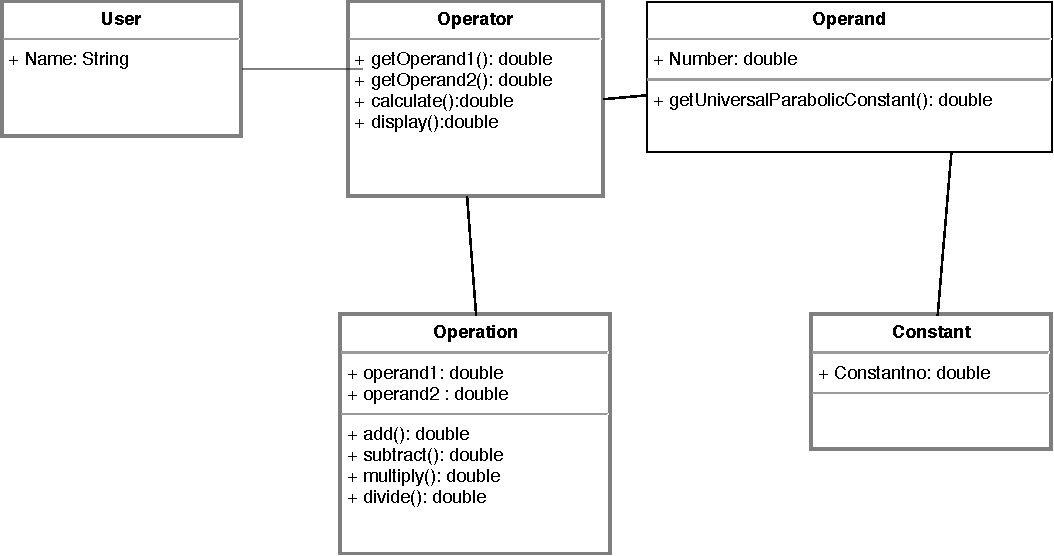
\includepdf[pages=1]{domain.pdf}
\newpage
\section{Description}
A calculator has 4 operators which are Add, Subtract, Multiply, Divide.
\subsection{User}
A user is a person who is using the calculator.
\subsection{Operator}
A user can use an operator to perform his calculation.\newline

\subsection{Operand}
Operand class shall be used to get all the irrational number. 
\subsection{Operation}
Addition, subtraction, multiplication and division are performed by this class.

\subsection{Constant}This class is for the Universal parabolic constant.


\bibliographystyle{plain}
\bibliography{references}
\end{document}